\chapter{Výpočet objemu - var. 1}
%Hlavní komponentou vyvíjeného systému je váha, kdy z naměřené hmotnosti jsme schopni vypočítat objem. Základní vztah pro výpočet objemu kapaliny je:
Hlavní komponentou vyvíjeného systému je váha, kdy z naměřené hmotnosti jsme schopni vypočítat objem. Použijeme základní vztah pro výpočet objemu, kde hmotnost kapaliny vypočítáme jako rozdíl plné a prázdné láhve:

\begin{equation}
    V = \frac{m}{\rho} \, \left[\mathrm{m^3}\right] \label{objem_kapalina}
 \end{equation}

V ...objem kapaliny

m ...hmotnost kapaliny \([\mathrm{kg}]\)

\(\rho\) ...hustota kapaliny \([\mathrm{kg/m^3}]\)
\\
\\
Výpočet hustoty kapaliny:

%V prvním případě je nutné vypočítat hmotnost kapaliny:

%\begin{equation}
%    m = m_{plná} - m_{prázdná} \, \left[\mathrm{kg}\right]
%    \label{objem_kapalina}
%\end{equation}

%\(m_{min}\) ...hmotnost prázdné láhve \([\mathrm{kg}]\)

%\(m_{max}\) ...hmotnost plné láhve \([\mathrm{kg}]\)
%\\

\begin{equation}
    \rho = \frac{m_{max} - m_{min}}{V_{max}} \, \left[\mathrm{kg/m^3}\right] \label{objem_kapalina}
\end{equation}

\(m_{min}\) ...hmotnost prázdné láhve \([\mathrm{kg}]\)

\(m_{max}\) ...hmotnost plné láhve \([\mathrm{kg}]\)

\(V_{max}\) ...objem plné láhve \([\mathrm{m^3}]\)
\\

%KOMENT

Při výpočtu objemu můžeme zanedbat tepelnou roztažnost ze dvou důvodů:

1)
Při inventarizaci se snažíme zjistit rozdíl v množství destilátu od předchozí inventury. Běžnou praxí je využití odměrného válce, kdy objem určujeme podle rysky. Nový systém však využívá nepřímého měření založeného na hmotnosti. Kapalina při změně objemu nemění svou hmotnost, což vyvolává otázku, proč se nesoustředíme na měření zbytkové hmotnosti místo objemu. V obchodní praxi, a to i v gastronomii, se však všechny lihoviny uvádějí v jednotkách objemu. Proto je nutné naměřenou hmotnost přepočítat na objem, přičemž je klíčové, aby všechny hodnoty byly vztaženy ke stejné teplotě, aby bylo možné výsledky mezi sebou porovnávat. 

Objem se počítá pro referenční teplotu, při které byl stanoven objem plné láhve. Každý kapalný produkt (nápoje, mycí prostředky, oleje atd.) uvádí na své etiketě objem, který je obvykle vypočítán pro pokojovou teplotu 20 °C. Výhodou této metody je, že umožňuje zjistit zbytkové množství kapaliny při jakékoliv teplotě. V případě odměrných válců by bylo nutné měřit všechny destiláty při pokojové teplotě, což je časově náročné(z důvodu než se nám alkohol vytažený z lednice zahřeje na pokojovou teplotu) nebo by bylo potřeba měřit teplotu lihoviny a následně provést korekční výpočet, jaký objem by kapalina měla při pokojové teplotě. Ani jeden z těchto postupů se však běžně nepoužívá kvůli své nepraktičnosti.

2)
V případě odměrných válců jejich nevýhodou je tepelná roztažnost kapalin, kdy válce jsou dimenzované pro konkrétní teplotu, obvykle 20 °C. Většina otevřených destilátů je chlazena v lednicích pro zachování chuti, kvality a aromatu, což způsobuje menší objem naměřený na válci oproti skutečnému. Podmínky skladování si stanovuje každý výrobce lihovin sám. Obvykle čím má lihovina menší procento alkoholu tím se podává chladnější, není to ale pravidlo. Víno je chlazeno na 5 - 15 °C, lihoviny 5 - 18 °C(gin, rum, whisky) a emulzní likéry(vaječný likér, Baileys) > 5 °C.

Například, měří-li se při teplotě 5 °C destilát s vysokým obsahem alkoholu, např. 80\% z důvodu vyšší tepelné roztažnosti ethanolu oproti vodě a při počátečním objemu 1 l, vyjde chyba 13,74 ml za předpokladu, že destilát obsahuje pouze ethanol a vodu bez dalších příměsí. Pro účely inventury však není tato chyba nijak významná. Postup výpočtu je ukázán níže. [\ref{objem_kapalina}]

\begin{equation}
\label{objem_kapalina}
    \Delta V = \Delta V_v + \Delta V_e \left[m^3\right]
\end{equation}


\[\Delta V = 0,64 + 1,13 = 13,74 \left[ml\right]\]


\(\Delta V\) ...celkový rozdílový objem

\(\Delta V_{v}\) ...rozdílový objem vody \([m^3]\)

\(\Delta V_{e}\) ...rozdílový objem ethanolu \([m^3]\)


\begin{equation}
%\label{objem_kapalina}
    \Delta V_v = \frac{p_v}{100} \cdot V_0 \cdot \beta_v \cdot (t_1 - t_0)
\end{equation}

\[\Delta V_v = \frac{20}{100} \cdot 1 \cdot  2,14 \cdot 10^{-4} \cdot (20 - 5) = 0,64 \left[ml\right]\]

\(p_v\) ...objemový podíl vody \([\%]\) 

\(V_0\) ...počáteční objem lihoviny \([m^3]\)

\(\beta_v\) ...součinitel objemové teplotní roztažnosti vody \([\frac{m^3}{m^3 \cdot ^\circ C}]\)

\(t_1\) ...koncová teplota \([^\circ C]\)

\(t_0\) ...počáteční teplota \([^\circ C]\)

\begin{equation}
    \Delta V_e = \frac{p_e}{100} \cdot V_0 \cdot \beta_e \cdot (t_1 - t_0)\left[m^3\right] \label{objem_kapalina}
\end{equation}

\[\Delta V_e = \frac{80}{100} \cdot 1 \cdot  1,09 \cdot 10^{-3} \cdot (20 - 5) = 13,1 \left[ml\right]\]

\(p_e\) ...objemový podíl ethalonu(alkoholu) \([\%]\) 

\(\beta_e\) ...součinitel objemové teplotní roztažnosti ethalonu \([\frac{m^3}{m^3 \cdot ^\circ C}]\)



%\begin{equation}
%    \rho = \frac{m_{plná} - m_{prázdná}}{V_{max}} \, \left[\mathrm{kg/m^3}\right] \label{objem_kapalina}
%\end{equation}


%Výsledný vzorec pro výpočet objemu:

%\begin{equation}
%    V = \frac{m - m_{prázdná}}{\rho} \, \left[\mathrm{m^3}\right] \label{objem_kapalina}
%\end{equation}

%%%%%%%%%%%%%%%%%%%%%%%%%%%%%%%%%%%%%%%%%%%%%%%%%%%%%%%%%%%%%%
%%%%%%%%%%%%%%%%%%%%%%%%%%%%%%%%%%%%%%%%%%%%%%%%%%%%%%%%%%%%%%
\chapter*{Výpočet objemu - var. 2}
\addcontentsline{toc}{chapter}{Výpočet objemu - var. 2}
Hlavní komponentou vyvíjeného systému je váha, kdy z naměřené hmotnosti jsme schopni vypočítat objem. Použijeme základní vztah pro výpočet objemu, kde hmotnost kapaliny vypočítáme jako rozdíl hmotnosti láhve se zbytkovou kapalinou a hmotnosti prázdné láhve:

\begin{equation}
    V = \frac{m - m_{min}}{\rho} \, \left[\mathrm{m^3}\right] \label{objem_kapalina}
\end{equation}

V ...objem kapaliny

m ...hmotnost láhve se zbytkovou kapalinou \([\mathrm{kg}]\)

\(m_{min}\) ...hmotnost prázdné láhve \([\mathrm{kg}]\)

\(\rho\) ...hustota kapaliny \([\mathrm{kg/m^3}]\)
\\
\\
Výpočet hustoty kapaliny:

\begin{equation}
    \rho = \frac{m_{max} - m_{min}}{V_{max}} \, \left[\mathrm{kg/m^3}\right] \label{objem_kapalina}
\end{equation}


\(m_{max}\) ...hmotnost plné láhve \([\mathrm{kg}]\)

\(V_{max}\) ...objem plné láhve \([\mathrm{m^3}]\)
\\
\\
Při výpočtu objemu můžeme zanedbat tepelnou roztažnost ze dvou důvodů:
\\
\begin{enumerate}
    \item
    Při inventarizaci se snažíme zjistit rozdíl v množství destilátu od předchozí inventury. Běžnou praxí je využití odměrného válce, kdy objem určujeme podle rysky. Nový systém však využívá nepřímého měření založeného na hmotnosti. Kapalina při změně objemu nemění svou hmotnost, což vyvolává otázku, proč se nesoustředíme na měření zbytkové hmotnosti místo objemu. V obchodní praxi, a to i v gastronomii, se však všechny lihoviny uvádějí v jednotkách objemu. Proto je nutné naměřenou hmotnost přepočítat na objem, přičemž je klíčové, aby všechny hodnoty byly vztaženy ke stejné teplotě, aby bylo možné výsledky mezi sebou porovnávat.
    
    Objem se počítá pro referenční teplotu, při které byl stanoven objem plné láhve. Každý kapalný produkt (nápoje, mycí prostředky, oleje atd.) uvádí na své etiketě objem, který je obvykle vypočítán pro pokojovou teplotu 20 °C. Výhodou této metody je, že umožňuje zjistit zbytkové množství kapaliny při jakékoliv teplotě. V případě odměrných válců by bylo nutné měřit všechny destiláty při pokojové teplotě, což je časově náročné(z důvodu než se nám alkohol vytažený z lednice zahřeje na pokojovou teplotu) nebo by bylo potřeba měřit teplotu lihoviny a následně provést korekční výpočet, jaký objem by kapalina měla při pokojové teplotě. Ani jeden z těchto postupů se však běžně nepoužívá kvůli své nepraktičnosti.
    
    \item 
    %Z výše uvedeného bodu vyplývá, že vypočítaný objem bude odpovídat referenční teplotě 20 °C. Stejně jako v příkladu č. [\ref{objem_kapalina}] se objeví zanedbatelná chyba, pokud bude měřicí systém stejně nebo přesnější než odměrný válec.
    I pro případ, kdybychom nepočítali objem pro referenční teplotu, tak odchylka vyjde stejně jako v příkladu č. [\ref{objem_kapalina}], kde se objeví zanedbatelná chyba, pokud bude měřicí systém stejně nebo přesnější než odměrný válec.
\end{enumerate}

%%%%%%%%%%%%%
\\ 
\\
Velkou výhodou výpočtu objemu přes hmotnost je eliminace vlivu tepelné roztažnosti, která nemá vliv na hmotnost

Nově navrhovaný měřící systém je navrhovaný z důrazem na rychlost měření a i když přesnost je sekundární z důvodu hrubého odhadu, tedy zda není např. odcizena lahev. Stejně do měření objemu destilátů vstupuje hromada drobných chyb, které těžko v praxi jsme schopni ovlivnit jako je
\begin{itemize}
    \item Nedodržení risky na panáku - ve spěchu přelijeme
    \item Rozlévání chlazeného alkoholu(menší objem), i když riska je dimenzovaná pro 20°C
    \item U alkoholu s nalévačem dochází k zvětrávání a vypařování ethanolu
    \item samotné chyby při inventůře viz kapitola výše
\end{itemize}

\section{Chyby měření}
Podle první kapitoli víme, že inventura je intrení zaležtostí podniku, pro kterou není nutné mít certifikované měřidla. Bylo by tedy dobré aby nový měřící systém měřil ser stejnou nebo i lepší přesnotí než stávající metody, tedy odměrné válce. Tedy pro určení přesnosti je nutné znát chyby které působí na měřící systém.
\subsection{Vliv tlaku}
Vliv tlaku obecně zanedbáváme, protože má téměr nulový vliv a to i otevřených válců, kde vztlaková síla vytlačí vzduch, vytlačený vzduch pak nemá žádný vliv. Při vážení lahví jsou lahve uzavřené, tak k vytlačení vzdchu nedochází pokud nemáme na hrdle nalévátko. Dále máme tlak co působi zvnějšku lahve, tedy při vychlazené lahvi dojde k ochlazení okolního vzduchu, který způsobí 

\subsection{Vliv teploty}
I když výhodou nepřímého výpočtu objemu přes hmotnost je eliminace vlivu tepelné roztažnosti, stále se teplota může projevit ve formě orosení lahve, kde dojde ke změně její hmotnosti.

Orosení neboli kondenzace vody na těle láhve je zapříčiněno rozdílem teplot a okolní vlhkostí. Klíčový je rosný bod (RB), který lze zjistit z rovnice rosného bodu[\ref{rosný bod obecne}], kde pro 20°c prostředí a vlhkost 50\% (běžně se pohybuje 40 - 60\%) vychází RB kolem 9,3 °C [\ref{rosný bod}], což je dostačující pro vyvolání osorosení u lahvích chlazených na 5°C. [z1][z2]
%FRYML, Martin. Návrh přístroje pro přímé stanovení rosného bodu.
%https://cs.wikipedia.org/wiki/Rosn%C3%BD_bod

\begin{equation}
T_{ds} = \frac{243,5 \cdot ln(\frac{V}{100} \cdot e^{\frac{17,67 \cdot T}{243,5 + T}})}{17,67 - ln(\frac{V}{100} \cdot e^{\frac{17,67 \cdot T}{243,5 + T}})}
\label{rosný bod obecne}
\end{equation}

\(T_{ds}\) ...Rosný bod \([\mathrm{^\circ C}]\)

\(V\) ...Relativní vlhkost vzduchu \([\mathrm{\%}]\)

\(T\) ...Teplota vzduchu \([\mathrm{^\circ C}]\)

\begin{equation}
T_{ds} = \frac{243,5 \cdot ln(\frac{50}{100} \cdot e^{\frac{17,67 \cdot 20}{243,5 + 20}})}{17,67 - ln(\frac{50}{100} \cdot e^{\frac{17,67 \cdot 20}{243,5 + 20}})} = 9,27
\label{rosný bod}
%\caption{Rovnice rosného bodu}
\end{equation}
\\
Dále na velikost orosení má vliv:
\begin{itemize}
    \item Velikost lahve - Čím větší plocha, tím více vysrážené vody.
    \item Obsah láhve - Přímo nijak neovlivňuje rosný bod, ale tekutina uvnitř udrží déle lahev chladnou, což zapříčiní více vysrážené vody.
\end{itemize}

Byl tedy proveden experiment na 3 lahvích různých objemů a obsahu kapaliny vychlazených na 5 °C v prostorách s teplotou 20 °C a relativní vlhkostí 53 \%. Než se naakumuluje dostatek vody na povrchu lahve chvilku to trvá, proto byla hmotnost lahve měřena po dobu 60 min. Níže tabulka ukazuje výsledky měření, kdy nejvyšší nárust byl 0,54 g po 30 min, po této době už hmotnost lahve začala klesat na svoji původní hodnotu.

%Byl tedy proveden experiment na 3 lahvích různých objemů a obsahu kapaliny vychlazených na 5 °C v prostorách s teplotou 20 °C a relativní vlhkostí 53 \%. Než se naakumuluje dostatek vody na povrchu lahve chvilku to trvá, proto byla hmotnost lahve měřena po dobu 60 min. V praxi se zbytkový objem odměřuje krátce po vytažení lahve, tudíš je validní brat v potaz výsledky v krátkém intervalu. Níže tabulka ukazuje výsledky měření, kde po 5 min jsme byly schopni naměřit rozdíl 0,5g a nejvyšší nárus byl 1g po 45 min, po této době už hmotnost lahve klesala zpět na původní hodnotu.

\begin{figure}[H]
    \begin{center}
        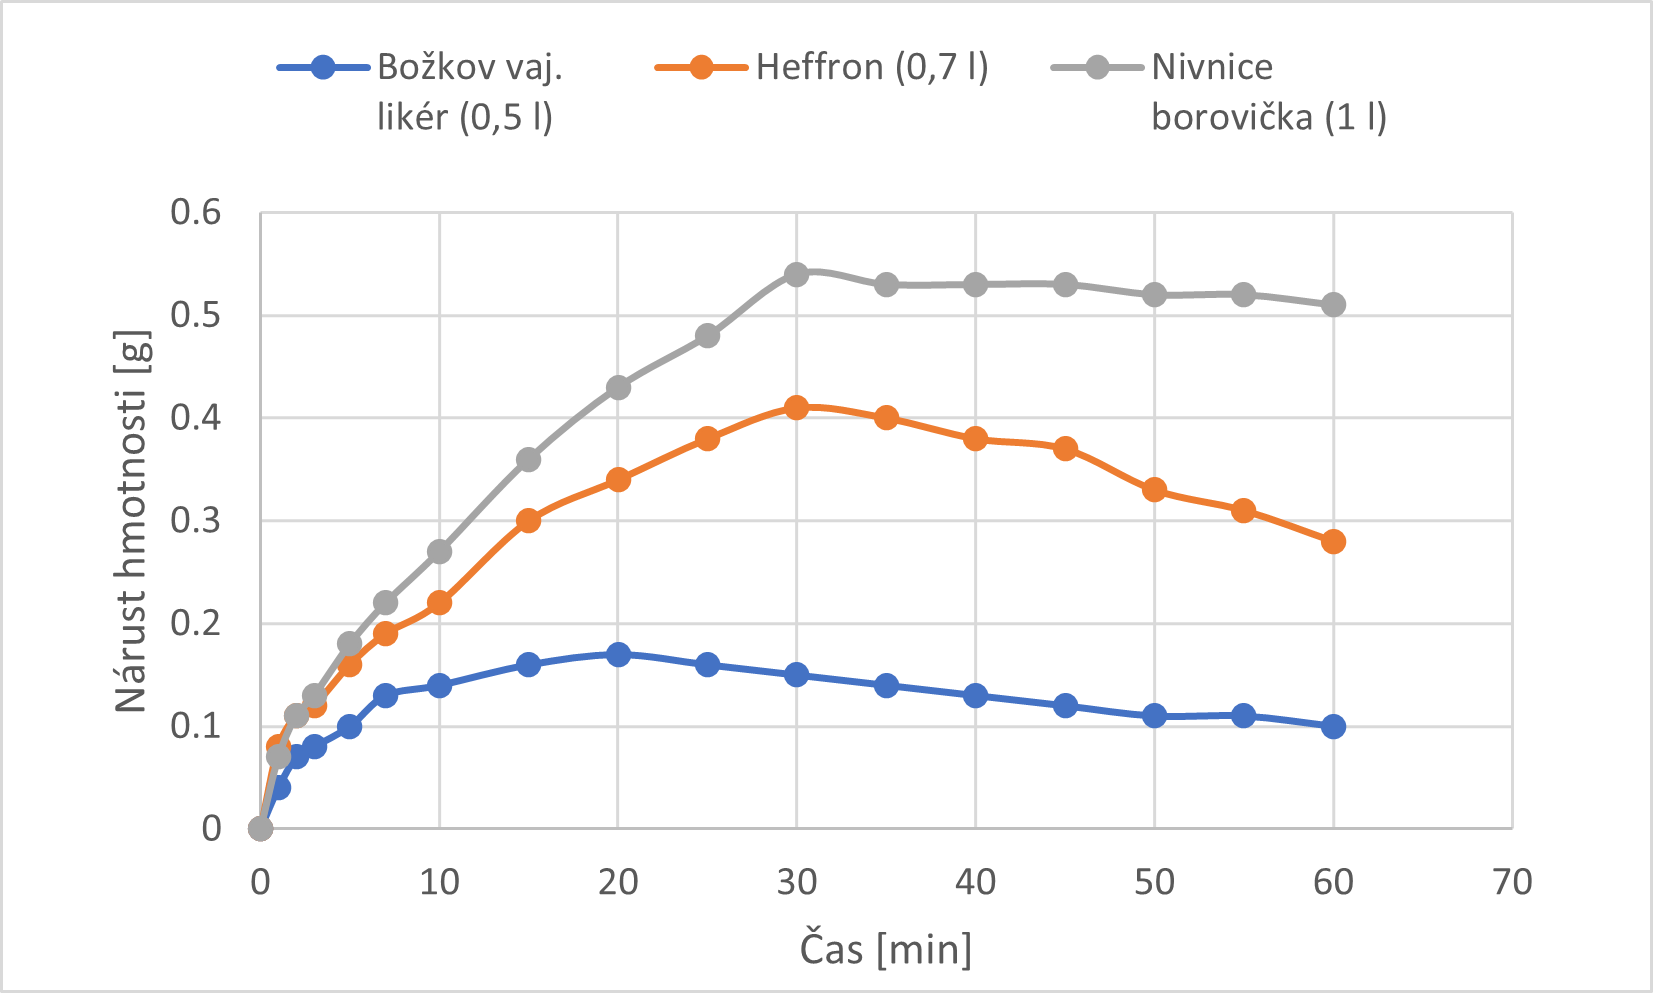
\includegraphics[scale=1.2]{obrazky/orosení.png}
    \end{center}
    \caption{Nárůst hmotnosti při orosení láhve}
\end{figure}


\begin{table}[H]
    \centering
    \begin{tabular}{|c|c|c|c|c|}
        \hline
         Destilát & \begin{tabular}[c]{@{}c@{}}Materiál \\ lahve [g]\end{tabular} & \begin{tabular}[c]{@{}c@{}}Objem \\ lahve [l]\end{tabular} & čas [min] & \begin{tabular}[c]{@{}c@{}}max. přírustek \\ hmotnosti [g]\end{tabular}\\
         \hline
         Nivnice bor. & Sklo & 1 & 30 & 0,54\\
         \hline
         Heffron (rum) & Sklo & 0,7 & 30 & 0,41\\
         \hline
         Božkov (vaječný lik.) & Sklo & 0,5 & 20 & 0,17\\
         \hline
    \end{tabular}
    \caption{Přírůstky hmotnosti při orosení láhve. Měřeno s přesností na 0,01 g.}
    \label{tab:my_label}
\end{table}

%V případě měření s přesnější váhou by nám výsledné přírustky hmotnosti vykreslili xxx charakter[xx]

V případě omezení této chyby stačí láhev před měřením otřít. Cílem, ale bylo ukázat jak vysoká chyba může nastat pokud lahev neotřeme. Pro praktické/provozní účely je tato chyba však zanedbatelná.

\subsection{Chyba hmotnosti lahve}
Jednou z chyb je možná odlišná hmotnost lahví při výrobě, proto bylo provedené měření rozdílu hmotností jednotlivých lahví. Pro ověření chyby z hmotnosti lahvi byla vybrána jeden z těžších destilátů. Testovných kusů bylo 15 lahví stejného typu a odlišných šarží. U stejných šarží je možné dosáhnout menší odchylky hmotnosti z důvodu identických podmínek výroby pro všechny lahve. 
Maximální rozptyl byl 3,5 g, tedy chyba +-, což u měření vody je schopno zpusobit chybu o velikosti 3,5 ml. Do výpočtu za hodnotu m\_min se bude uvádět průmerná hodnota ze všech naměřených lahví.


\subsection{Chyba hmotnosti nalévače}
Některé láhve mají na svém hrdle nalévač nebo také nalévátko místo víčka, který ulehčuje rozlévání alkoholu. Jeho hmotnost se pohybuje na základě typu, lehčí nalévače jsou menší a plastové s hmotností od xx, na druhé straně máme nalévače větší celokovové, který váží až xx. Hmotnost samotného nalévače přináší chybu do měřeného systému, proto bude kompenzovaná databázi hmotností jednotlivých nalévačů. Dalším řešením je nalévač před měřením sundat, to ale zpomaluje vykonání inventury.   

\subsection{Chyby hustoty}

Pro výpočet objemu je nutné znát hustotu destilátu[xx]. Hustota lze stanovit dvoumi způsobi z hlediska přesnosti a časové náročnosti.

%Za předpokladu, že by uživatel chtěl sám doplnit databázi o nový produkt, je nutné pro výpočet hustoty dodat m-max, m-min a V-max dle vzorečku[xx]. Problém je, že dle legislativy ISOxxx v rámci obchodního řetězce může dodavatel dodat 

Navážením plné lahve a pro tuto hmotnost stanovit maximální objem dle etikety. Zde ale do systému přichází chyba objemu. Dle normy xxx jsou tekuté produkty v obchodním řetězci mít dovolenou chybu z objemu max. 15\% tedy pro 1l lahev to dělá 15 ml, což způsobuje větší nepřesnost než odměrné válce. Tato metoda je sice není tolik přesná, ale usnadňuje uživateli evidovat novou lahev do databáze.

Druhou možností je evidovat lahev pomocí odměrného válce vyšší přesnosti než je požadována pro měřící systém tedy delta\_V < +-5ml. Tato metoda už není tolik uživatelský přívětivá, protože kombinuje další zařízení, ale jedná pouze o jednorázovou činnost. Válce se navíc cenově pohybují do 1000 kč, což na jednorázovou investici není teké moc, otázkou je zda uživatel stojí o vylepšení o 10 ml například.

Nejlépe by se dal tento problém vyřešit znemožněním evidence uživateli do databáze a člověk

Cílem práce je mít databázi uloženou na serveru, kde si uživatel váhy pouze stahne aktualizovanou databázi, kde je evidovaná hustota destilátu s maximální přesností pro minimalizaci chyby, ale chci dát též uživateli možnost si uložit destilát do databáze za předpokladu, že by měl exotický kousek který by nebyl uloženy v databazi na serveru a to za cenu snížení přesnosti měření tohoto destilátu. 

Poslední možností je, pokud uživatel trvá na vysoké přesnosti a destilát neni uložen v databázi je možné si pořídit vlastní přesné zařízení pro stanovení hustoty kapaliny jako je pyknometr nebo přesná váha + přesný odměrný válec.

Cílem zařízení je i cenově dostupná možnost pro řešení inventarizace, proto do online databáze budou ukládaná s přesností, která neovlivní výslednou přesnost zařízení. Obsluhu a správu online databáze bude provádět prodejce měřícího systému (já).

proto je jednodušší do systému evidovat hustotu naměřenou přesnějším měřidlem, tedy stačí odměrný válec



%Navážením plné lahve a pro tuto hmotnost stanovit maximální objem dle etikety. Zde ale do systému přichází chyba objemu. Dle normy xxx jsou tekuté produkty v obchodním řetězci mít dovolenou chybu z objemu max. 15\% tedy pro 1 l lahev to dělá 15 ml, což způsobuje větší nepřesnost než odměrné válce, pokud by uživatel upřednostňoval vyšší přesnost je zde druhá možnost evidence a to pomocí odměrného válce s přesností 0,5 ml na 100 ml. Tímto způsobem navíc eliminujeme chybu z hmotnosti lahve[xx], který by se za normálních okolností přičetl k chybe objemu

\subsection{Chyba váhy}
Posledním klíčovým faktorem je chyba váhy. Teoreticky by nám stačila přesnost vyšší jak +-10g (+-10 ml vody), ale je nutné vzít v potaz i ostaní chyby, které ve výsledku mohou překročit celkovou chybu +-10 ml. Tedy přesnost váhy musí být určena z ohledem na to aby měřící systém jako celek nepřekročil celkovou chybu +-10ml.

Hmotnost se nám ve vzorci vyskytuje na 3 místech: m, m-min a m-max. Z praktického hlediska bude měření těchto veličin prováděno stejnou váhou.

\subsection{Stanovení přesnosti váhy na základě }
%Propagace nejistot pro měřící metodu A
\subsection{Výpočet hustoty přes hmotnost lahve a stanovení přesnosti váhy}

Zde dominantní chybu tvoří objem kapaliny, i když nám z měření vyšla chyba pouze +-xx ml, tak budem počítat z maximálně možnou dle normy ISOXXX.

Výslednou chybu dokáže ovlivnit zda m\_min a m\_max budem měřit ze stejné láhve či nkoli. v případě stejné láhve se nám vykompenzuje chyba způsobená rozptylem hmotností lahví (+- 0,85g)

I když chyba systému je zanedbatelná pro inevnturní účely v praxi bude systém připojen k online databázi, aby uživatel nemusel vést databízi a ukládat do ní nové destiláty, možnost toho ale zustane pro případ uložení destilátu, který nebude dostupný v rámci online databáze, tam budou hustoty destilátů měřeny s maximální přesností(jednorázová investice), důvodem je jednorázová investice, která se finančně nijak nedotýka spotřebitele a navíc hlavním zdrojem chyby systému je právě ze stanovená hustoty, pro minimalizaci chyby. Přesnost váhy zůstane stejná z důvodu pořizovacích nákladů (není důvod si připlácet o několik tisíc korun za možnost naměřit objem o "3 kapky" lépe / není důvod si připlácet o několik tisíc korun za možnost naměřit objem s přesností na 0,01 ml). V případě zanedbání chyby hustoty by celková chyba systému vyšla 


\[\Delta V = \Delta m + \Delta m_m + \Delta m_r = +- 2 ml\]


\begin{figure}[H]
    \begin{center}
        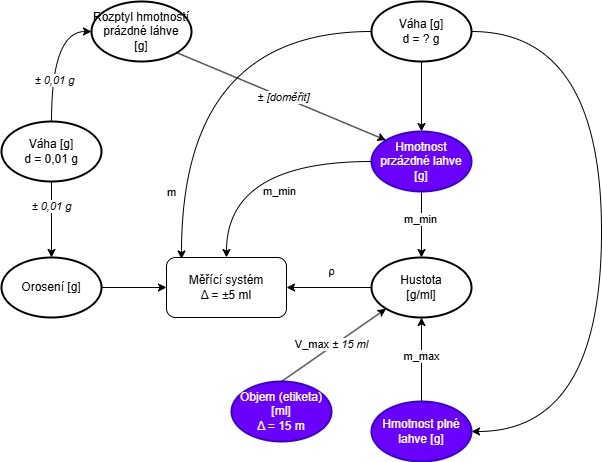
\includegraphics[scale=0.6]{obrazky/Propagace nejistot-Metoda1+.jpg}
    \end{center}
    \caption{Propagace nejistot - Výpočet hustoty pomocí plné láhve}
\end{figure}

\subsection{Výpočet hustoty pomocí odměrného válce a stanovení přesnosti váhy}

V tomto případě, bude stanovení objemu pro výpočet hustoty prostřednictím odměrného válce, který bude dostačující přesnosti, aby celý systém splňoval kritérium přesnosti. Přesnost válce a váhy by vůči sobě neměly být příliš rozdílný, aby měli na chybu stejný vliv (ovlivnily chybu ve stejném řádu - tedy se nejlépe navzájem vyrovnají). (pokud válec bude větší přesnosti a váha menší, přesnost válce bude automaticky kompenzována na přesnost váhy a naopak.). Dostupné válce na trhu se řídí zmíněnou normou ISOxxx. Podmínkou výběru válce je absolutní chyba pod +-5ml, tedy válce s menším objeme. Z dostupných válcu na trhu je nejvhodnějším kadinátem 250 ml válec s přesností +-1ml, kde jeho relativní chyba činí 0,4\% tedy jedná se o nejpřesnější válec na velikost vlastního objemu. Tedy pokud budem stanovovat hustotu ze vzorku pokrývající max objem válce a váhou stejné přesnosti výjde nám nejmenší relativní chyba hustoty.

Požadovaná přesnost váhy závisí na hustotě měřené kapaliny. Čím hustší kapa-
linu máme, tím menší přesnost vyžadujeme, a naopak - méně hustá kapalina bude
vážit méně na jednotku objemu, v našem případě 10 ml. Tudíž nás zajímá, která
složka destilátu má nejmenší hustotu. Ve své podstatě bude měřen pouze ethanol
a voda, co se týče příměsí pro dochucení, tak ty jsou větší hustoty, proto přesnost váhy vztáhneme k ethanolu, i když nikdy nebudeme měřit 100\% ethanol, ale jeho směs s vodou a dalšími příměsi.

Nakonec byl vytvořen Python script, který kombinuje dotupné přesnosti odměrných válců a vah. Z důvodu, jak bylo zmíněné už u válce nezáleží na absolutní chybě ale relativní, tudíž je možné využít celé spektrum dostupných válců, které se relativně jen mírně liší, díky skriptu ne že jsem schopen najít nejpřesnější kombinaci, ale vidím všechy ostatní kombinace pro přehled a jak působí na měřící systém.

\begin{equation}
    \pm m = \pm 5 \cdot 0.789 \, \left[\mathrm{g}\right] \label{objem_kapalina}
\end{equation}



%Metoda výpočtu hustoty využívá odměrný válec jako objemový etalon. Aby výsledná kombinovaná nejistota metody nepřekročila požadované ± 5 ml, musí být nejistoty jednotlivých měřidel (válec × váha) zvoleny tak, aby se na celkové nejistotě podílely přibližně stejnou měrou.
%Graduované válce dostupné na trhu se vyrábějí podle ČSN EN ISO 4788 (třídy přesnosti A a B). Pro třídu A platí např. tyto maximální dovolené odchylky:


\begin{figure}[H]
    \begin{center}
        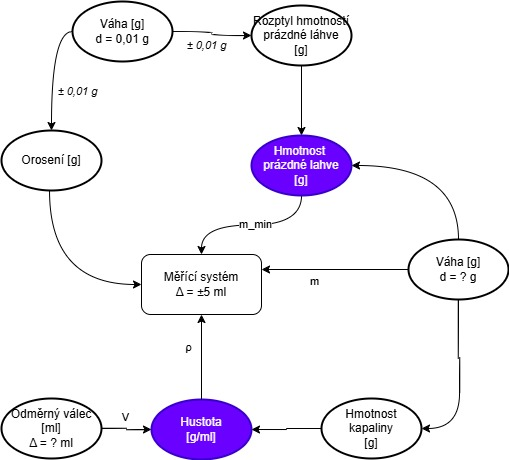
\includegraphics[scale=0.6]{obrazky/Propagace nejistot-Metoda 2+.jpg}
    \end{center}
    \caption{Propagace nejistot - Výpočet hustoty pomocí odměrného válce}
\end{figure}

%---------------------------------------------------------------
%  Výpočet kombinované nejistoty objemu plněné lahve
%  Metoda 2 (jedna váha + odměrný válec) – číslované kroky 1–7
%---------------------------------------------------------------

\section{Výpočet kombinované nejistoty (metoda 2)}

%--------------------------------------
\subsection*{Přehled použitých veličin}
\begin{center}
\begin{tabular}{>{$}c<{$} l l}
\toprule
\text{symbol} & \text{hodnota} & \text{poznámka}\\
\midrule
\rho              & 0{,}998\;\text{g\,ml}^{-1} & voda při 20\,$^\circ$C\\
V_{\mathrm{nom}}  & 1\,000\;\text{ml}          & jmenovitý objem lahve\\
V_{\mathrm{válec}}& 250\;\text{ml}             & třída A, ISO 4788\\
\Delta_{\mathrm{válec}} & \pm 1\;\text{ml}      & MPE válce (Max.~Permissible Error)\\
\Delta           & \pm 0{,}01\;\text{g}        & tolerance váhy (společná pro $m_\text{tot}$, $m_\text{min}$, $m_\rho$)\\
\sigma_{\text{lahve}} & 1{,}0\;\text{g}        & směrodatná odchylka hmotností prázdných lahví\\
\bottomrule
\end{tabular}
\end{center}

%--------------------------------------
\subsection{Krok 1 – Převod tolerancí na standardní nejistoty}

\begin{align}
u_{\text{váha}}
      &= \frac{\Delta}{\sqrt{3}}
       = \frac{0{,}01\;\text{g}}{\sqrt{3}}
       \approx 0{,}0058\;\text{g},\\
u_{\text{válec}}
      &= \frac{\Delta_{\text{válec}}}{\sqrt{3}}
       = \frac{1\;\text{ml}}{\sqrt{3}}
       \approx 0{,}577\;\text{ml}.
\end{align}

%--------------------------------------
\subsection{Krok 2 – Nejistoty hmotností měřených touž vahou}

\[
u_{m_\text{tot}} = u_{m_\text{min}} = u_{m_\rho}=u_{\text{váha}}.
\]

%--------------------------------------
\subsection{Krok 3 – Nejistota hmotnosti kapaliny v lahvi}

\begin{align}
u_{m_\text{kap}}
  &= \sqrt{u_{m_\text{tot}}^{2}
        +\bigl(u_{m_\text{min}}^{\,2}+\sigma_{\text{lahve}}^{2}\bigr)} \\[2pt]
  &= \sqrt{(0{,}0058)^2 +\bigl((0{,}0058)^2 + 1{,}0^2\bigr)}\;\text{g} \\
  &\approx 1{,}000\,03\;\text{g}\;\;(\text{zaokrouhleno}\;1{,}00\;\text{g}).
\end{align}

%--------------------------------------
\subsection{Krok 4 – Nejistota hustoty vzorku}

\begin{align}
m_\rho^{\text{nom}}
  &= V_{\text{válec}}\rho
   = 250 \times 0{,}998
   = 249{,}5\;\text{g},\\[4pt]
u_\rho
  &= \rho \sqrt{\Bigl(\frac{u_{m_\rho}}{m_\rho^{\text{nom}}}\Bigr)^2
                 +\Bigl(\frac{u_{\text{válec}}}{V_{\text{válec}}}\Bigr)^2} \\[4pt]
  &= 0{,}998 \sqrt{\Bigl(\frac{0{,}0058}{249{,}5}\Bigr)^2
                   +\Bigl(\frac{0{,}577}{250}\Bigr)^2} \\[4pt]
  &\approx 0{,}0020\;\text{g\,ml}^{-1}.
\end{align}

%--------------------------------------
\subsection{Krok 5 – Propagace na objem lahve}

\begin{align}
u_V
  &= \sqrt{\Bigl(\frac{u_{m_\text{kap}}}{\rho}\Bigr)^2
           +\Bigl(V_{\text{nom}}\frac{u_\rho}{\rho}\Bigr)^2} \\[4pt]
  &= \sqrt{\Bigl(\frac{1{,}00}{0{,}998}\Bigr)^2
           +\Bigl(1\,000 \times \frac{0{,}0020}{0{,}998}\Bigr)^2} \\[4pt]
  &\approx 2{,}57\;\text{ml}.
\end{align}

%--------------------------------------
\subsection{Krok 6 – Rozšířená nejistota}

Použijeme koeficient pokrytí $k=2$ (přibližně 95~\%):

\[
U_{95} = k\,u_V = 2 \times 2{,}57 \approx 5{,}14\;\text{ml}.
\]

%--------------------------------------
\subsection{Krok 7 – Shrnutí}

Výsledná rozšířená nejistota měření objemu 1 l lahve \textbf{metodou 2}  
při váze $\pm0{,}01$ g a válci 250 ml ±1 ml (třída A) je

\[
\boxed{U_{95} \approx \pm 5{,}1\ \text{ml}},
\]

což splňuje stanovené kritérium \mbox{$U_{95}\le \pm 5$ ml} s nepatrnou rezervou.


%%%%%%%%%%%%%%%%%%%%%%%%%%%%%%%%%%%%%%%%%%%%%%%%%%%%%%%%%%%%%%
%%%%%%%%%%%%%%%%%%%%%%%%%%%%%%%%%%%%%%%%%%%%%%%%%%%%%%%%%%%%%%

%\chapter*{Přepočet hmotnosti na objem}
%\addcontentsline{toc}{chapter}{Přepočet hmotnosti na objem}
%\label{Přepočet hmotnosti na objem}
%Přepočet hmotnostního množství na objemové / Výpočet objemu
%\section{Princip}

%Hlavní komponentou vyvíjeného systému je váha, která slouží, stejně jako víše zmíněne váhy, k přepočtu hmotnostního množství na objemové.
%Ze známe hmnotnosti 

%Hlavní komponentou vyvíjeného systému je váha, která slouží k přepočtu hmotnostního množství na objemové. Základní vztah pro výpočet objemu je: 

%Hlavní komponentou vyvíjeného systému je váha, kdy z naměřené hmotnosti jsme schopni vypočítat objem. Základní vztah pro výpočet objemu kapaliny je:

%\begin{equation}
%    V = \frac{m}{\rho} \, \left[\mathrm{m^3}\right] \label{objem_kapalina}
%\end{equation}

%V ...objem kapaliny

%m ...hmotnost kapaliny \([\mathrm{kg}]\)

%\(\rho\) ...hustota kapaliny \([\mathrm{kg/m^3}]\)
%\\

%V praxi by byla tato metoda poměrně přesná pro výpočet objemu pouze čirých destilátů, které mají složení “jen” vody a ethanolu, pro které známe hustotu a poměr mezi nimi, díky známé hodnotě obsahu alkoholu. Barevné destiláty nebo destiláty s vyšší viskozitou obvykle obsahují další příměsi, pro které neznáme jejich hustotu a poměr mezi nimi a výpočet pouze z vody a ethanolu by vedl na velkou chybovost.
%Tato metoda by byla v praxi poměrně přesná pro výpočet objemu pouze čirých destilátů, které se skládají "jen" z vody a ethanolu. Pro tyto destiláty známe hustotu a poměr obou složek díky známému obsahu alkoholu. Barevné nebo viskózní destiláty však obvykle obsahují další příměsi, jejichž hustotu a poměr neznáme. Výpočet pouze z vody a ethanolu by proto vedl k velké nepřesnosti.

%\section{Linearizace}
%\label{odkazos}
%https://cs.wikipedia.org/wiki/ISO_1
%https://cs.wikipedia.org/wiki/Standardn%C3%AD_teplota_a_tlak

%Pro výpočet objemu kapaliny, v našem případě destilátů, můžeme za určitých podmínek použít linearizaci dvou bodů. Výpočet provedeme ze známého objemu plné láhve a hmotnosti prázdné a plné láhve. Teplota a tlak nemají vliv na hmotnost, tedy na množství alkoholu, a proto je můžeme zanedbat. Výsledný objem bude platit pro referenční teplotu a tlak, při kterých byl stanoven objem plné láhve.

%Výpočet objemu kapaliny v našem případě destilátů se dá za určitých podmínek spočítat pomocí linearizace dvou bodů %- hmotnosti prázné a plné lahve a k tomu patřičný objem.

%Výpočet budem provádět ze známého objemu plné láhve a naměřené hmotnosti prázdné a plné láhve. Teplota a tlak nemá vliv na naměřenou hmotnost tedy množství alkoholu a můžeme je zanedbat. Výsledný objem bude pro referenční teplotu a tlak při které byl stanoven objem plné láhve. %Pro naše účely tedy není nutné znát objem v daném okamžiku, ale za  

%Tuhle teplotu a tlak stanovuje česká norma ČSN EN ISO 1 (01 4110).

%Výpočet je tedy závislý na naměřené hmotnosti na kterou nemá vliv teplota ani tlak. 

%Tím, že je výpočet závislý na hmotnosti, tak můžeme zanedbat teplotu a tlak. Rozdílem hmotností kapaliny a láhve jsme schopni získat  

%Teplotu a tlak můžeme zanedbat. Tím, že měříme hmotnost 

%Při fyzické inventuře nás zajímá skutečné množství  


%V našem případě tlak v uzavřené láhvi je tak malý, že neovlivňuje výsledný objem kapaliny. Teplota 

%inventurní účely se dá  
%
%však můžem použít jinou metodu, která není závislá na hustotě, tedy teplotě a tlaku s tím spojená. 
%
%%Hustota je závislá na teplotě, proto budem počítat s její referenční hodnotou teploty. Budem předpokládat, jaký 
%%Našim cílem je po
%
%Hustota je závislá na teplotě a tlaku. V případě kapalin můžeme tlak zanedbat z důvodu "nulového" vlivu na výsledný objem.
%
%V praxi
%
%Hustota je závislá na teplotě a tlaku, proto si stanovíme pevnou hodnotu teploty, kterou budem považovat za konstantu. Budem tedy počítat objem kapaliny pro referenční teplotu a tlak. Náš objem tedy bude závisly pouze na hmotnosti a můžeme ho linearizovat.
%
%Našim cílem je změřit objem alkoholu bez nutnosti jej přelévat, proto budem měřit i hmotnost lahve ve kterém se alkohol nachází. Ze známe hmotnosti prázdné "m1" a plné láhve "m2 "a tomu příslušnému objemu 'V2', jsme schopni vytvořit předpis přímky ze dvou bodů. %V první řadě je nutné zjistit směrnici (pro nulový offset):

%Výpočet objemu pomocí předpisu přímky ve směrnicovém tvaru:
%\begin{equation}
%    V = k \cdot m - q\, \left[\mathrm{m^3}\right] \label{objem_linearizace}
%\end{equation}

%Výpočet směrnice:
%\ref{objem_linearizace}
%\begin{equation}
%    k = \frac{V_{max}-V_{min}}{m_{max}-m_{min}}\, \left[\mathrm{m^3/kg}\right]\label{směrnice}
%\end{equation}

%\(V_{min}\) ...objem prázdné láhve \([\mathrm{m^3}]\)

%\(V_{max}\) ...objem plné láhve \([\mathrm{m^3}]\)

%\(m_{min}\) ...hmotnost prázdné láhve \([\mathrm{kg}]\)

%\(m_{max}\) ...hmotnost plné láhve \([\mathrm{kg}]\)
%\\

%Objem prázdné lahve bude vždy nulový, proto můžeme předpis směrnice zjednodušit:
%\begin{equation}
%    k = \frac{V_{max}}{m_{max}-m_{min}}\, \left[\mathrm{m^3/kg}\right] \label{směrnice_ez}
%\end{equation}

%Pokud to nepujde napsat vizuálně zlomkovým tvarem, tak dat nezapomenout závorky

%Výpočet offsetu:
%\begin{equation}
%    q = V_{min} - k \cdot m_{min}\, \left[\mathrm{m^3}\right] \label{offset}
%\end{equation}

%Opětovně jde zjednodušit na tvar:

%\begin{equation}
%    q = k \cdot m_{min}\, \left[\mathrm{m^3}\right] \label{offset_ez}
%\end{equation}

%Pro naší aplikaci bude V1 vždy rovna nule, protože minimální objem je nulový

%%FOTO grafu ve kterem bude Vmin = 0

%\section{Linearizace}